We have run a handful of tightly-controlled experiments. Rather than a
list of results, let us draw the \textbf{capability map}: one picture
that says, for each behavior we tested, whether the model acquired it,
whether it generalizes, what it costs, and where it breaks.

We record each finding with an honest epistemic label --- what is
\emph{proven} (measured), what is \emph{supported}, what is
\emph{suggestive}, and what is \emph{unknown}.

\section{Why a map, and not a single
score}\label{why-a-map-and-not-a-single-score}

There is a strong temptation, at the end of an investigation, to reach
for one number and say ``that's the verdict.'' It would be satisfying
and simple. But every experiment in this book has argued against exactly
that. The model is good at some things and terrible at others, and those
are both true at once. A single number would have to collapse them, and
collapsing them would hide the most important thing: the \emph{shape} of
the boundary.

So we draw a map instead. A map does not pretend to be one verdict; it
shows \emph{dimensions}. It answers, for each question we asked, what we
found --- and, crucially, what we did \emph{not} find. That honesty
about the unknown is what makes the map worth more than a headline.

\section{The four-level generalization
map}\label{the-four-level-generalization-map}

\begin{figure}
\centering
\pandocbounded{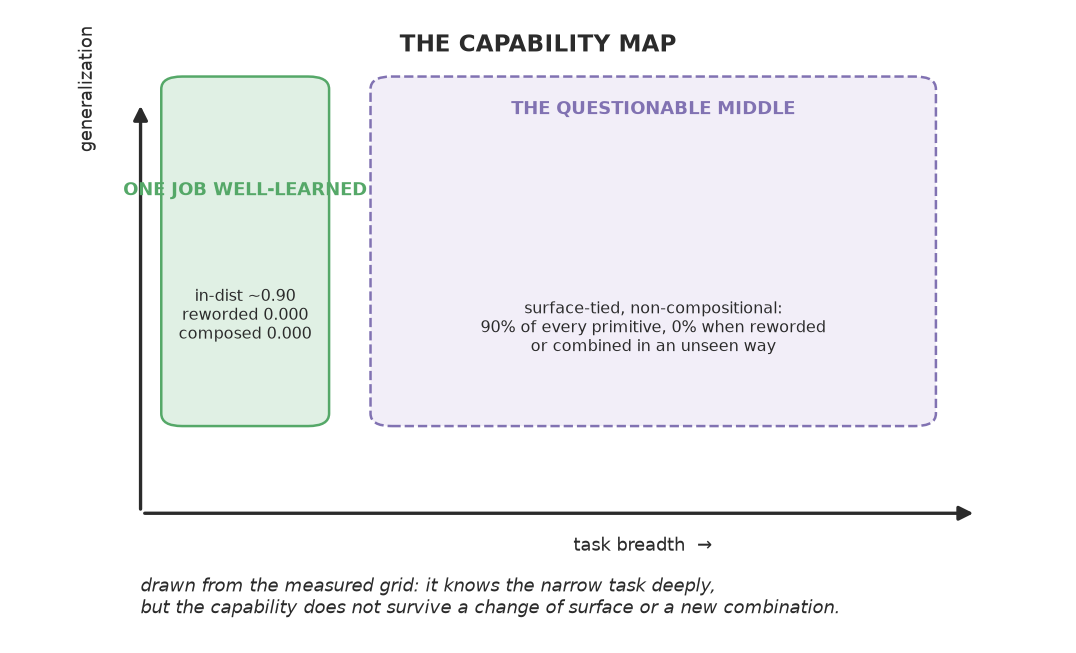
\includegraphics[keepaspectratio,alt={The capability map},width=\maxwidth{\textwidth},keepaspectratio]{figures/fig_capability_map.png}}
\caption{The capability map}
\end{figure}

The map puts the measured grid on two axes: the breadth of tasks and the
depth of generalization. The narrow job is well-learned; the broader
ground is not.

Recall the four levels from Chapter 2. Here is what we measured at each,
on the \textasciitilde0.9M model:

\begin{longtable}[]{@{}
  >{\raggedright\arraybackslash}p{0.1400\linewidth}
>{\raggedright\arraybackslash}p{0.2800\linewidth}
>{\raggedright\arraybackslash}p{0.3400\linewidth}
>{\raggedright\arraybackslash}p{0.1600\linewidth}
@{}}
\toprule\noalign{}
\begin{minipage}[b]{\linewidth}\raggedright
Level
\end{minipage} & \begin{minipage}[b]{\linewidth}\raggedright
The question
\end{minipage} & \begin{minipage}[b]{\linewidth}\raggedright
Measured result
\end{minipage} & \begin{minipage}[b]{\linewidth}\raggedright
Status
\end{minipage} \\
\midrule\noalign{}
\endhead
\bottomrule\noalign{}
\endlastfoot
\textbf{L1 Mem} & Can it be explained by remembering? & Held-out 59/60;
canary → general program & \texttt{{[}PROVEN{]}} it generalizes
primitives, doesn't parrot \\
\textbf{L2 Dist} & Does it work on new instances of the same task? &
In-distribution 0.900 & \texttt{{[}PROVEN{]}} yes \\
\textbf{L3 Surf} & Does it survive superficial change? & New wording →
0.000; new identifiers → 0.350 & \texttt{{[}PROVEN{]}} no ---
surface-tied \\
\textbf{L4 Struct} & Can it compose known pieces in unseen ways? & 0.000
(baselines also 0.000) & \texttt{{[}PROVEN{]}} no \\
\end{longtable}

This is the map's spine. Read it vertically and it shows a steady
decline in how much we can trust the model's ``understanding'' as we
move from ``did it see this before'' (Level 1) to ``can it put things
together'' (Level 4). The model passes the first two levels cleanly and
fails the last two completely. That is the boundary we keep coming back
to.

\section{The scaling map (what changes
it)}\label{the-scaling-map-what-changes-it}

\begin{longtable}[]{@{}
  >{\raggedright\arraybackslash}p{0.1731\linewidth}
>{\raggedright\arraybackslash}p{0.1979\linewidth}
>{\raggedright\arraybackslash}p{0.5690\linewidth}
@{}}
\toprule\noalign{}
\begin{minipage}[b]{\linewidth}\raggedright
Lever
\end{minipage} & \begin{minipage}[b]{\linewidth}\raggedright
Tested
\end{minipage} & \begin{minipage}[b]{\linewidth}\raggedright
Effect on composition
\end{minipage} \\
\midrule\noalign{}
\endhead
\bottomrule\noalign{}
\endlastfoot
Model size & 0.88M → 29.3M (\textasciitilde33×) & \textbf{none} ---
still 0.000 at all four sizes \\
Data size & 100 → 3000 examples & helps \emph{in-distribution}
(0.10→0.64), not composition \\
Training protocol & sequential vs replay & \textbf{big} --- fixes
continual retention (0.000→1.000) \\
\end{longtable}

The second half of the map is about levers, and it is where the
surprising findings live. We tried three ways to move the composition
boundary --- more capacity, more data, and a different training
procedure. Two of them did nothing to composition, and one of them was
the decisive lever for a \emph{different} problem (continual learning).
This asymmetry is worth circling, because it tells us where effort does
and does not pay.

\section{What's proven vs.~what's
unknown}\label{whats-proven-vs.-whats-unknown}

\textbf{Proven (measured, this setup):} - The model learns single
operations to \textasciitilde90\% in-distribution and generalizes them
across instances (L1/L2). - It is surface-tied: new wording → 0.000, new
identifiers → 0.350 (L3). - It cannot compose: unseen combinations →
0.000, and neither \textasciitilde33× capacity (across 0.88M→29.3M) nor
more data changes this (L4). - Continual learning is a procedure
problem: sequential forgets (A → 0.000), replay retains (A → 1.000) with
no acquisition cost. - The pilot task was retrieval-solvable (retrieval
= 1.000), so that split is ``too easy''; the composition split is not
(all baselines 0.000).

\textbf{Supported / suggestive:} - The composition failure is likely
\emph{structural-data} (exposure to combinations), not capacity --- but
we did not test feeding the model compositions directly, so this is
suggestive.

\textbf{Unknown (did not test):} - Whether feeding composites during
training unlocks composition. - Whether behavior on 3+ capabilities or
post-continual composition holds. - Human-written task transfer
(recommended external sanity check, not yet run). - Whether a
fundamentally different inductive bias (not scale) helps.

\section{The boundary, in one line}\label{the-boundary-in-one-line}

\begin{quote}
\textbf{A small model learns narrow, individual mappings well and
generalizes them across instances, but its knowledge is surface-tied and
non-compositional --- and within the tested range, neither more
parameters nor more data nor a different training order turns that into
robust, compositional capability.}
\end{quote}

\section{Why the map is the
deliverable}\label{why-the-map-is-the-deliverable}

This map is the book's real output. It is not a single headline accuracy
that would mislead; it is a precise, honest picture of where capability
exists, where it collapses, and what (and what doesn't) shift the
boundary. It is the answer to the central question --- and it is
falsifiable, built from real measured runs, and honest about what
remains unknown.

The deeper value of the map is what it does to our confidence. Before
drawing it, we knew ``the model is limited.'' After drawing it, we know
\emph{precisely which limits are structural} (composition,
surface-tiedness --- not moved by scale or data) and \emph{which are
procedural} (continual forgetting --- fixed entirely by how we train).
That distinction between structural and procedural limits is the kind of
knowledge that changes what a practitioner would try next. It is not the
same as saying ``small models are weak''; it is saying ``here is exactly
where the weakness lives, and here is what does and does not reach it.''

That precision, not a dramatic narrative, is the honest payoff of the
whole brew. And it is why we are willing to state as an \emph{unknown}
the questions we did not answer, rather than fill the map with confident
guesses. A map with a blank region is more useful than a map painted
over with speculation, because the blank marks where the next
investigation should go.
